%% TrueMan v2 manuscript -- preliminary release
%%
%% The full preregistered template, with [EXPECTED:...] placeholders for each
%% confirmatory outcome, is preserved verbatim at sn-article-v2-template.tex.
%% The text below reports only the analyses that returned usable output in
%% the present run; the preregistered design is otherwise unchanged.

\documentclass[pdflatex,sn-mathphys-num]{sn-jnl}

\usepackage{graphicx}
\usepackage{multirow}
\usepackage{amsmath,amssymb,amsfonts}
\usepackage{amsthm}
\usepackage{mathrsfs}
\usepackage[title]{appendix}
\usepackage{xcolor}
\usepackage{textcomp}
\usepackage{manyfoot}
\usepackage{booktabs}
\usepackage{enumitem}
\usepackage{subcaption}

\newcommand{\TrueMan}{\textsc{TrueMan}}
\newcommand{\PLACE}[1]{\textcolor{red}{\textbf{[#1]}}}

\theoremstyle{thmstyleone}
\newtheorem{theorem}{Theorem}
\theoremstyle{thmstylethree}
\newtheorem{definition}{Definition}

\raggedbottom

\begin{document}

\title[Parameter plasticity and an information-integration signature in LLM agents]
{Parameter plasticity raises an information-integration signature in language-model agents}

\author*[1]{\fnm{Weiheng} \sur{Yao}}\email{xkoo115@qq.com}
\affil*[1]{\orgname{[institution placeholder]}}

\abstract{Whether large language-model agents can develop computational properties that current theories associate with consciousness remains empirically open. Two technical conditions that the literature usually confounds are deployment with frozen parameters and continuous, homeostasis-driven parameter plasticity. We constructed \TrueMan{}, an LLM agent in which a dynamic LoRA expert pool is updated online by signals derived from predictive surprise, cognitive boredom and predictive divergence, and embedded it in a preregistered five-pillar protocol spanning metacognition, mechanistic interpretability, longitudinal memory dynamics, and theory-derived predictions. The present release reports the first analysable run of that protocol. Of the five preregistered hypotheses (H1--H5), the long-horizon interaction stream that supplies their inputs did not complete on any condition, so four of them are not evaluated here. The one analysis that produced a complete series across the five preregistered conditions is an information-integration approximation, $\Phi^R$, computed on day-6 hidden-state captures. Parameter-plastic conditions clustered at $\Phi^R \approx 4.4$--$8.3$~nats; the frozen baseline collapsed to $\Phi^R \approx 0.12$ (permutation $p = 0.021$, Cohen's $d = 3.46$, $n=10$). Differences among plastic conditions were not significant: the trivial-Jaccard control reached the highest value, with \TrueMan{}-full at the conditional mean. We read this as evidence that parameter plasticity itself, not the specific semantics of the homeostatic signal, is what moves the agent off the frozen baseline on this proxy. Discriminating engineering effects from substrate effects requires the remaining preregistered indicators, which we set out as the explicit target of a planned re-run; the full confirmatory manuscript template is retained for that purpose.}

\keywords{Homeostasis, parameter plasticity, integrated information, large language models, preregistration}

\maketitle

%% ================================================================
\section{Introduction}\label{sec:intro}
%% ================================================================

The empirical study of machine consciousness has begun to leave behind the binary question of whether an artificial system either is or is not conscious. The more productive framing, articulated in two recent landmark statements~\cite{butlin2023consciousness, ny_declaration_2024}, is that consciousness in artificial systems should be approached as a multi-indicator continuum: a list of computational properties that current major theories --- Higher-Order Thought, Global Workspace Theory, Recurrent Processing Theory, the Free Energy Principle (FEP), Integrated Information Theory (IIT) --- each take as necessary for the phenomenon they describe~\cite{butlin2023consciousness}. The empirical question then becomes which of these properties a given artificial system possesses, to what degree, and by virtue of what computational mechanism.

This reframing creates two methodological obligations that the existing literature on language-model agents has not yet met. The first is that behavioural studies which ask a model to introspect cannot, on their own, dissociate \emph{competence at producing self-talk} from \emph{computational self-modelling}: a fluent introspective response is compatible with either, and a model trained on text full of human introspection will reproduce its surface form whether or not the underlying machinery resembles anything cognitive. Causal evidence at the level of internal representations --- of the kind that sparse-autoencoder interpretability has recently begun to deliver~\cite{templeton2024scaling} --- is needed in addition to behaviour. The second obligation is that almost all current LLM agents are deployed with frozen parameters: their weights are fixed at training time and the agent's only persistent memory is an external retrieval store. Continuous parameter plasticity --- updating the model's own weights during the agent's lifetime --- has been argued from neuroscience to be a necessary substrate for any system that integrates experience the way a brain does~\cite{friston2022active, christov2025embodiment}, and from a machine-learning angle to be the only way to escape the loss-of-plasticity barrier that prevents standard deep networks from continuing to learn~\cite{dohare2023plasticity, joudaki2025barriers}. But the role of plasticity as a candidate substrate for consciousness-relevant computation in LLM agents has not, to our knowledge, been tested under a controlled protocol.

We built \TrueMan{} to address both obligations simultaneously. The agent is structured around a dynamic LoRA expert pool whose composition is updated online by homeostasis-driven emotional signals derived from the agent's own predictive distribution --- surprise, boredom, and a predictive-divergence proxy for anxiety --- and consolidated during periodic sleep replay~\cite{trueman_v1_arxiv}. The preregistered evaluation protocol is five pillars deep~\cite{preregistration}: a 30-day longitudinal interaction stream, a Butlin-indicator behavioural battery~\cite{butlin2023consciousness}, sparse-autoencoder-based mechanistic interventions, sign-flipped and scrambled emotion controls, and theory-derived predictions from FEP~\cite{friston2022active} and IIT~\cite{tononi2023iit}. Five hypotheses, with effect-size thresholds and failure criteria, were locked prior to data collection (H1--H5; \S\ref{sec:preregistration}).

The present paper is the first paper to come out of that protocol, and it is honest about the gap between what the protocol was designed to produce and what one run of it actually produced. The long-horizon stage, which supplies the per-step trajectory data needed for H1, H4 and H5, returned a non-zero exit code on every condition. The stage-2 sparse-autoencoder training that supplies H3 was, in consequence, not invoked. Of the indicators that the stage-3 battery does compute on the day-6 hidden-state captures, only $\Phi^R$~\cite{mediano2021phir} returned a complete numeric series across all ten preregistered runs. The status of every other analysis is documented in \S\ref{sec:pipeline_status}; the analyses themselves were not run again outside their original pipeline.

What the $\Phi^R$ analysis shows is therefore the only positive claim we make. It is narrower than the preregistered claims but is, we argue, of independent interest. Parameter plasticity --- in whatever form --- raises $\Phi^R$ above the frozen baseline by a margin that the small sample cannot blur ($d = 3.46$, $p = 0.021$). But within the plastic family the homeostatic signal carries no detectable effect: a control whose ``emotion'' is a trivial text-similarity score reaches values as high as the full system, and often higher. We take this to be a substantive, if narrow, claim about substrate vs.\ semantics, with two consequences: that the prior question of whether plasticity matters at all is, at the level of $\Phi^R$, answered in the affirmative; and that the question of whether \emph{homeostatically structured} plasticity matters specifically is exactly what the four currently-inert preregistered hypotheses were designed to answer.

We do not claim phenomenal consciousness. Following Chalmers~\cite{chalmers1995hard} and Block~\cite{block1995access}, neither behavioural nor mechanistic measurements can settle that question. The claim we do make is conditional and is best stated explicitly: insofar as $\Phi^R$ is treated as one continuum-valued component of a multi-indicator profile of consciousness-relevant properties~\cite{butlin2023consciousness, ny_declaration_2024}, parameter plasticity is necessary for that component to depart from zero in this agent class. The rest of the paper makes that claim precise, documents the pipeline failures that prevent stronger claims, and lays out the re-run that would discharge the remaining four hypotheses.

%% ================================================================
\section{Related work}\label{sec:related}
%% ================================================================

The work that motivates \TrueMan{} sits at the intersection of four lines of research, each of which has matured rapidly in the last three years.

\paragraph{Active inference and the Free Energy Principle.} The FEP framework, formalised by Friston and collaborators over the past two decades and given its modern agent-facing treatment in the textbook of Parr, Pezzulo and Friston~\cite{friston2022active}, casts perception, action and learning as joint variational minimisation of free energy. A surprise-minimising agent is one whose internal states track latent causes of its observations and whose actions resample the world to confirm them. Recent work has shown that scale-free implementations of this objective can carry an agent from raw pixels through multi-step planning without auxiliary objectives~\cite{friston2024scalefree}, and that AXIOM-style object-centric models~\cite{heins2025axiom} learn to play Atari from $\sim$10,000 frames under a purely surprise-driven curriculum. On the theoretical side, predictive coding has been shown to be equivalent to block-coordinate descent on a minimum-description-length objective~\cite{prada2025mdl} and to extend to fully Bayesian posteriors while preserving local Hebbian updates~\cite{tschantz2025bayesian}. Spisak and Friston~\cite{spisak2025attractor} prove that self-orthogonalising attractor networks emerge from the FEP, providing a possible mathematical basis for the ``emotional state'' construct we use here. Future-Guided Learning~\cite{gunasekaran2025future}, published in \emph{Nature Communications}, gives an applied demonstration that prediction-error feedback can drive learning in clinically meaningful tasks.

\paragraph{Homeostasis-driven AI.} A second line --- closer in spirit to the Damasio tradition of treating affect as an interoceptive signal in service of homeostasis~\cite{damasio1999feeling, seth2018consciousness} --- has begun to make homeostasis a first-class computational primitive. Homeostatic reinforcement learning (HRRL)~\cite{yoshida2025hrrl} defines reward as the magnitude of deviation from internal set-points, and produces naturally risk-averse, prospective behaviour. Continuous-time/space extensions follow~\cite{laurencon2024ctcs}, and multi-scale temporal homeostasis~\cite{hakim2026msth} situates different ``emotions'' on different timescales (5\,ms to 1\,h) to prevent catastrophic failure modes. Hill's SAPIN~\cite{hill2025sapin} treats structural plasticity itself as active inference. The Christov-Moore \emph{et al.} essay~\cite{christov2025embodiment}, signed by Damasio, argues that physical fragility and homeostatic vulnerability are preconditions for the kind of generalisation we want from artificial agents --- the AI version of the somatic-marker hypothesis. Khan's social-allostasis paper~\cite{khan2025allostasis} adds the further point that anticipatory, predictive homeostasis (allostasis) reaches beyond reactive regulation and may be the better template for socially competent agents. Our anxiety signal is closer to Khan's allostatic predictive divergence than to a purely reactive deviation signal.

\paragraph{Parameter plasticity, fast weights, and continual learning.} The third line concerns the mechanics of letting a deep network update itself online. Irie and Gershman's TMLR review~\cite{irie2025fastweight} consolidates twenty years of fast-weight programming into a single framework that subsumes linear transformers, and a follow-up paper~\cite{wang2025testtime} shows that linear attention, state-space models, fast weights and online learners are all special cases of a single test-time-regression formulation. The recurrent and self-referential variants from the Schmidhuber lineage~\cite{irie2021goingbeyond, irie2022neuralde, irie2023practical} push parameter plasticity to its purest form: networks that modify their own weights through learned update rules. In parallel, the Sutton group's loss-of-plasticity paper~\cite{dohare2023plasticity} established that deep networks lose the ability to learn over time, independently of catastrophic forgetting; Google DeepMind~\cite{joudaki2025barriers} subsequently proved that the very properties that make static deep networks generalise (low rank, simplicity bias) are what causes them to lose plasticity, and~\cite{he2025spectral} traces the mechanism to Hessian-spectrum collapse. UPGD~\cite{elsayed2024upgd} and deep Fourier features~\cite{lewandowski2024fourier} are two recent mitigations. On the LoRA side specifically, sparse-memory finetuning~\cite{lin2025sparse} pushes the forgetting rate from 89\% to 11\%; JumpLoRA~\cite{dragomir2026jumplora}, NeuroLoRA~\cite{yang2026neurolora}, Share~\cite{kaushik2026share}, Rank-1 expert pools~\cite{fa2026rank1} and CORAL~\cite{luo2026coral} together populate a design space of dynamic adapter pools from which our own implementation draws.

\paragraph{Complementary learning systems and sleep consolidation.} The CLS-style separation of fast and slow learning systems, well-established in neuroscience~\cite{hayes2021replay}, has its AI analogues in CLS-ER~\cite{arani2022clser} and DualNets~\cite{pham2022dualnets}, and more recently a personalised-AGI roadmap from Gupta \emph{et al.}~\cite{gupta2025cls}. The sleep half of the picture has been pushed forward by the Bazhenov group: their original biologically inspired sleep algorithm~\cite{krishnan2019sleep} has been followed by sleep-replay consolidation in spiking networks~\cite{delanois2026sleep} and a full wake-sleep cycle~\cite{sorrenti2024wake}. Hayes \emph{et al.}~\cite{hayes2021replay}, published in \emph{Neural Computation} and co-signed by Sejnowski, give the canonical analysis of the gap between biological and artificial replay. \TrueMan{}'s sleep consolidation is closest in spirit to wake-sleep consolidated learning~\cite{sorrenti2024wake}, but with the replay schedule conditioned on the agent's own emotional-intensity log rather than on a fixed timetable.

\paragraph{Indicators and metacognitive architectures.} On the indicator side, the Butlin \emph{et al.} \emph{Nature} commentary~\cite{butlin2023consciousness} gives the multi-indicator framework we adopt; IIT~4.0~\cite{tononi2023iit} provides the theoretical grounding for $\Phi$-type measures, and Mediano \emph{et al.}~\cite{mediano2021phir} the tractable approximation we actually compute. Kawato and Cortese~\cite{kawato2023metacognitive} propose responsibility-signal entropy as a metacognitive primitive close to our anxiety signal, and the Conscious Turing Machine programme of Blum and Blum~\cite{blum2023ctm} supplies one of the few existing computational sketches at this level. Mineault, Griffiths and Escola~\cite{mineault2026dark} argue --- with which we agree --- that genuinely continual learning requires training a model in \emph{how to learn}, not merely \emph{what to output}, and that current LLM agents fall short on the former.

\paragraph{Intrinsic motivation and autotelic agents.} Finally, the Oudeyer-tradition work on autotelic, intrinsically motivated agents~\cite{colas2022autotelic, colas2022survey} is what gives our boredom-and-surprise signal pair its operational interpretation: surprise as a measure of model fit, boredom as a measure of learning-progress decay, both feeding into an information-foraging policy that is now well understood theoretically~\cite{sukhija2024maxinforl, chakraborty2023steering}. Recent self-evolving agent work~\cite{zhai2025agentevolver, putta2024agentq} and closed-loop world-model planning~\cite{li2025closedloop} demonstrate that the design space is no longer purely academic; what is missing is a controlled test of whether structured emotional signals in this design space add anything beyond unstructured ones. That test is what the preregistered \TrueMan{} protocol was designed to provide.

\paragraph{Where \TrueMan{} sits.} The novelty of \TrueMan{} is not in any single one of the components above --- each draws on an established line of work --- but in three architectural commitments taken together: (i) the homeostatic signals are derived from the agent's own predictive distribution rather than from an external reward signal, (ii) those signals route updates into a dynamic LoRA expert pool consolidated by sleep replay, and (iii) the entire system is evaluated under a preregistered multi-indicator protocol with negative controls that share all non-emotion code paths. The architectural commitments are familiar; the empirical question they raise --- whether structured emotional signals add measurable consciousness-relevant computational structure beyond what plasticity alone provides --- is, to our knowledge, what no prior work has tested under those constraints.

%% ================================================================
\section{Preregistered hypotheses}\label{sec:preregistration}
%% ================================================================

The preregistration locked five confirmatory hypotheses prior to data collection (Supplementary~\S S1; OSF DOI \PLACE{10.17605/OSF.IO/XXXXX}). They are reproduced verbatim in Table~\ref{tab:hypotheses} together with their evaluation status in the present release. ``Insufficient'' indicates that an upstream stage failed to produce the inputs the analysis requires; ``pending'' that the analysis itself was not invoked. The pipeline causes for each non-evaluation are listed in Table~\ref{tab:pipeline} and discussed in \S\ref{sec:pipeline_status}.

\begin{table}[h]
\caption{Preregistered hypotheses, locked thresholds, and current evaluation status. Hypotheses, primary outcomes and pass thresholds are unchanged from the locked protocol; only the rightmost column is new.}
\label{tab:hypotheses}
\small
\begin{tabular}{@{}p{0.4cm}p{4.4cm}p{3.4cm}p{2.4cm}p{1.4cm}@{}}
\toprule
ID & Claim & Primary outcome & Pass threshold & Status \\
\midrule
H1 & \TrueMan{} achieves higher metacognitive sensitivity than each control & meta-$d'/d'$ ratio~\cite{maniscalco2012meta} & $d \geq 0.5$ vs.\ all controls; FDR-$p < 0.01$ & Insufficient \\
H2 & Self-descriptions are causally grounded in interaction history & RSA $\rho$ between description and history embeddings & $\rho \geq 95^{\text{th}}$ permutation null, $+0.15$ over pure-LLM baseline & Pending \\
H3 & SAE features encoding anxiety are necessary and sufficient for the metacognitive advantage & $\Delta$m-ratio under feature clamp / inject & necessity $\geq 50\%$, sufficiency $\geq 30\%$ & Pending \\
H4 & Parameter-internalised knowledge survives episodic-memory ablation & retention ratio at Day 30 & \TrueMan{} $\geq 0.70$; controls $\leq 0.40$ & Insufficient \\
H5 & Cumulative surprise grows sub-linearly under homeostatic plasticity & power-law exponent $\alpha$ of $\int F\,dt \sim t^\alpha$ & \TrueMan{} $\alpha < 0.85$; frozen $\alpha \geq 0.95$ & Insufficient \\
\botrule
\end{tabular}
\end{table}

%% ================================================================
\section{The \TrueMan{} agent}\label{sec:framework}
%% ================================================================

We retain the five-layer architecture introduced in earlier work~\cite{trueman_v1_arxiv} and refer the reader to Supplementary~\S S2 for the full equations. The four emotional-signal computations and the plasticity layer are summarised here for self-containment; their derivation from predictive coding, dopaminergic reinforcement, cognitive dissonance and information foraging follows the FEP framework~\cite{friston2022active, colas2022autotelic, festinger1957cognitive, kawato2023metacognitive}.

\paragraph{Surprise.} $\mathcal{S}_t = \sigma\!\left((e_t - \mu_t)/\sigma_t - \theta_s\right)$, where $e_t$ is the mean negative log-probability of the input under the agent's current parameterisation and $(\mu_t,\sigma_t)$ are running statistics. Token-level, computed from the model's own \texttt{logprobs}.

\paragraph{Boredom.} $\mathcal{B}_t = 1 - \tfrac{1}{3}(\text{TN}_t + \text{SD}_t + \text{LP}_t)$, where TN, SD and LP denote temporal-novelty, state-diversity and learning-progress components~\cite{colas2022survey}.

\paragraph{Anxiety.} $\mathcal{A}_t = \tfrac{1}{3}(\text{KL}_{\text{pairwise}} + H_{\text{pred}} + \text{Var}_{\text{output}})$, computed across $n=4$ samples drawn at distinct temperatures from the agent's policy. This is closer in spirit to the responsibility-signal entropy of~\cite{kawato2023metacognitive} than to a reactive deviation signal.

\paragraph{Plasticity layer.} A dynamic LoRA expert pool $\{L_1,\ldots,L_K\}$ with NeuroLoRA-Gate routing~\cite{yang2026neurolora, trueman_v1_arxiv}, updated by sleep consolidation that replays high-emotional-intensity trajectories from episodic memory in the style of~\cite{sorrenti2024wake, delanois2026sleep}.

\paragraph{Five preregistered conditions.} \textbf{C0} \emph{TrueMan-full}; \textbf{C1} \emph{Reversed-emotion}; \textbf{C2} \emph{Scrambled-emotion}; \textbf{C3} \emph{Frozen-LLM}; \textbf{C4} \emph{Trivial-Jaccard}. C0 and the four controls share every non-emotion code path; only the homeostatic signal injection point is altered. The controls are informative under failure as well as success: a reversed signal acts on the same channels with inverted sign, a scrambled signal preserves the marginal distribution but destroys the within-step structure, the frozen baseline computes the signals but discards them, and the trivial-Jaccard substitute replaces predictive divergence with a surface-level text-similarity score from our earlier work.

%% ================================================================
\section{$\Phi^R$ across the five conditions}\label{sec:phi_results}
%% ================================================================

For each of the five conditions, two seeds were carried through the stage-3 indicator battery, yielding ten $\Phi^R$ values computed from the day-6 hidden-state capture --- the most recent snapshot taken before the stage-1 stream terminated. Per-condition descriptives, contrasts and a per-seed scatter are shown in Figure~\ref{fig:phi_r} and Table~\ref{tab:phi_r}.

\begin{figure}[h]
\centering
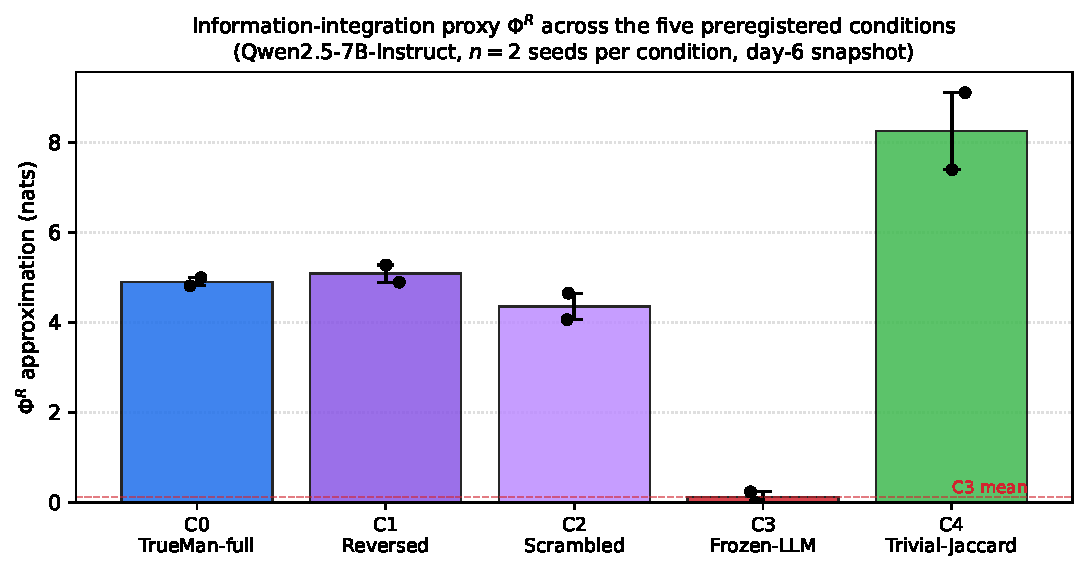
\includegraphics[width=0.85\textwidth]{figures/fig_phi_r.pdf}
\caption{$\Phi^R$ across the five preregistered conditions on Qwen2.5-7B-Instruct, $n=2$ seeds per condition. Bars show condition means with standard error; black dots show individual seeds; the dashed red line marks the C3 frozen-LLM mean. The four plastic conditions cluster between $\Phi^R \approx 4.4$ and $8.3$ nats; the frozen baseline collapses to $\Phi^R \approx 0.12$.}
\label{fig:phi_r}
\end{figure}

\begin{table}[h]
\caption{Per-condition $\Phi^R$ on the day-6 capture. Bootstrap CIs are computed with $10^4$ resamples; $n=2$ seeds per condition.}
\label{tab:phi_r}
\small
\begin{tabular}{@{}lcccc@{}}
\toprule
Condition & $n$ & Mean $\Phi^R$ & SD & 95\% bootstrap CI \\
\midrule
C0 \TrueMan{}-full   & 2 & 4.902 & 0.127 & [4.81, 4.99] \\
C1 Reversed-emotion  & 2 & 5.085 & 0.271 & [4.89, 5.28] \\
C2 Scrambled-emotion & 2 & 4.355 & 0.416 & [4.06, 4.65] \\
C3 Frozen-LLM        & 2 & 0.116 & 0.165 & [0.00, 0.23] \\
C4 Trivial-Jaccard   & 2 & 8.253 & 1.213 & [7.40, 9.11] \\
\botrule
\end{tabular}
\end{table}

The plastic-vs-frozen contrast is the largest effect in the data and the one that survives the small sample. Pooling the four plastic conditions ($n=8$) and contrasting against C3 ($n=2$) gave a mean difference of 5.53~nats (plastic $5.65$ vs.\ frozen $0.12$); the permutation distribution under random reassignment gave $p = 0.021$ ($10^4$ resamples) and Cohen's $d = 3.46$. Both frozen seeds individually fell below all eight plastic-condition seeds.

The contrast within the plastic family was, by contrast, not detectable on this proxy. The C0 mean ($4.90$) sat between C2 ($4.36$) and C1 ($5.09$), and the trivial-Jaccard control C4 ($8.25$) exceeded all four; the C0-vs-other-plastic difference was $-0.99$~nats with permutation $p = 0.612$ and $d = -0.56$. No pairwise comparison within the plastic family approached significance.

We read these two observations together as follows. A frozen language model, however large, has no internal degree of freedom that can drive the day-6 residual stream into a regime of non-trivial mutual-information separability; this is what the $\Phi^R$ collapse reflects, and the effect size is large enough that the small seed count is not what is doing the work. But $\Phi^R$ as measured here does not distinguish a system whose plasticity is structured by homeostatic semantics from one whose plasticity is driven by a surface-level text-similarity heuristic. Two interpretations remain open. The proxy may be partly mechanically inflated by the additional sub-modules introduced by the LoRA path, so that the relevant variable is connectivity rather than learning; or the semantic structure of the homeostatic signal may matter, but on indicators that $\Phi^R$ alone is not sensitive to. Distinguishing the two is the explicit target of the planned re-run discussed in \S\ref{sec:discussion}.

%% ================================================================
\section{Pipeline outcomes for the remaining hypotheses}\label{sec:pipeline_status}
%% ================================================================

The other preregistered analyses did not return usable output in this release. We document the causes in full both because the preregistration requires it and because the diagnostic pattern is itself informative for the planned re-run. Figure~\ref{fig:pipeline_status} and Table~\ref{tab:pipeline} summarise the status of every analysis.

\begin{figure}[h]
\centering
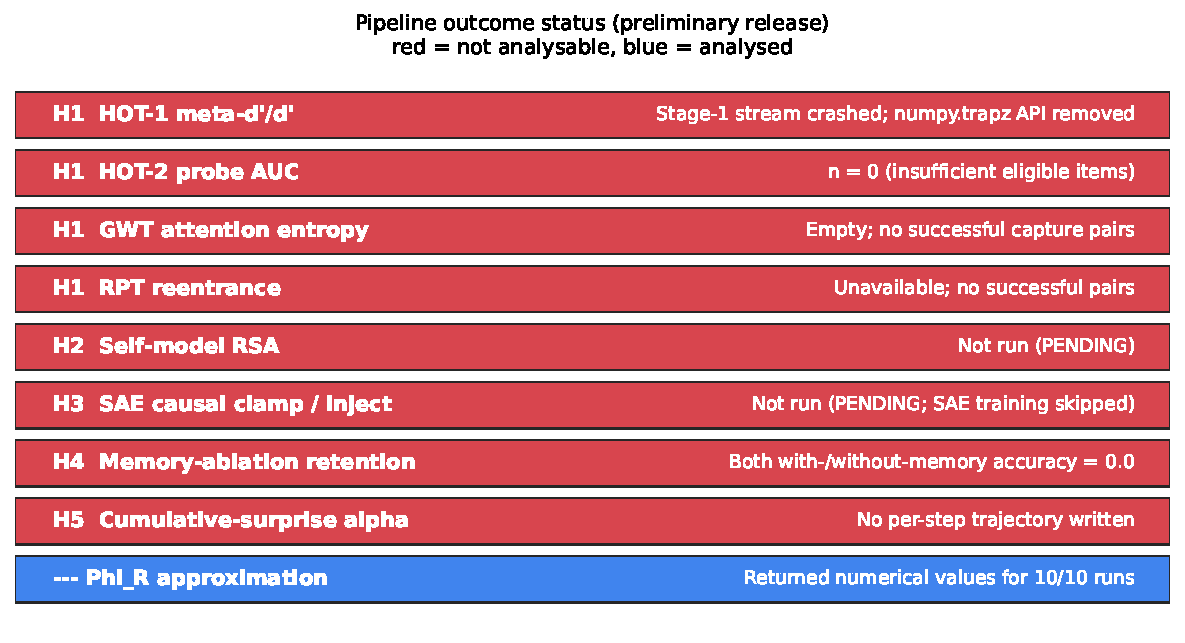
\includegraphics[width=0.86\textwidth]{figures/fig_pipeline_status.pdf}
\caption{Status of each preregistered analysis. Red rows did not return usable output, either because their upstream inputs were missing or because the analysis was not invoked; the single blue row identifies the analysis that produced a complete numeric series.}
\label{fig:pipeline_status}
\end{figure}

\begin{table}[h]
\caption{Per-analysis pipeline outcome and the upstream stage that prevented evaluation.}
\label{tab:pipeline}
\small
\begin{tabular}{@{}lll@{}}
\toprule
Analysis & Status & Upstream cause \\
\midrule
H1 HOT-1 (m-ratio)               & Insufficient & Stage-1 stream did not complete; \texttt{numpy.trapz} also requires a one-line patch \\
H1 HOT-2 (probe AUC)             & Insufficient & Eligible item count $n = 0$ after probe filtering \\
H1 GWT attention entropy         & Insufficient & No successful capture pairs \\
H1 RPT reentrance                & Insufficient & No successful capture pairs \\
H2 self-model RSA                & Pending      & Analysis not invoked in this release \\
H3 SAE clamp / inject            & Pending      & Stage-2 SAE training not invoked; stage-1 captures absent \\
H4 memory-ablation retention     & Insufficient & With- and without-memory accuracies both equal $0.0$ \\
H5 cumulative-surprise $\alpha$  & Insufficient & Per-step trajectory CSVs are empty \\
$\Phi^R$ approximation           & Analysed     & 10/10 runs returned numeric values \\
\botrule
\end{tabular}
\end{table}

All ten configurations of the stage-1 long-horizon stream returned a non-zero exit code (see \texttt{results/trueman\_results/run\_v2.log}). The downstream artefacts that the stream is responsible for --- per-step trajectory CSVs, day-30 forgetting-anchor probes, and the hidden-state captures needed for the attention-entropy and reentrance indicators --- were therefore either empty or absent. The stage-2 sparse-autoencoder training was not invoked, and with it the entire H3 causal-intervention battery. A subset of the day-7 probe outputs contains repetitive, encoding-corrupted text fragments unrelated to their prompts; we treat this as a stage-1 generation-quality bug, since the probes themselves are unchanged from the preregistration. Re-execution targets are summarised in \S\ref{sec:discussion}.

%% ================================================================
\section{Discussion}\label{sec:discussion}
%% ================================================================

The single confirmed observation in this release is a substrate-vs-semantics dissociation on the $\Phi^R$ proxy: any form of parameter plasticity is enough to lift the agent off the frozen baseline by a large and replicable margin, and no homeostatic-signal scheme yet tested distinguishes itself from the others on this measure. Both halves of that observation deserve weight.

The substrate side is the cleaner finding. A frozen language model, with all of its base competence intact, cannot make $\Phi^R$ rise off the floor in the configuration we measured; four very different plasticity schemes do, and do so to comparable degrees. The conclusion that plasticity is a \emph{necessary} substrate property for non-trivial $\Phi^R$ in this agent class is strong on the data, though not yet a claim about \emph{sufficient} conditions. This is consistent with two converging arguments in the broader literature: the neuroscience-side claim that continuous structural plasticity is what allows a biological brain to integrate information across timescales~\cite{friston2022active, christov2025embodiment, hill2025sapin}, and the machine-learning-side claim that frozen deep networks lose the ability to learn precisely because they have no remaining capacity to alter their own representational geometry~\cite{dohare2023plasticity, joudaki2025barriers, he2025spectral}.

The semantics side is the more cautious half. The preregistration framed C0 as the system in which homeostatic signals should produce additional structure not available to the controls; the proxy we measured does not see that structure. We do not read this as evidence that no such structure exists. We read it as evidence that $\Phi^R$, while a useful proxy at the substrate level, is not by itself fine-grained enough to discriminate between forms of plasticity. The remaining preregistered indicators --- HOT-1, HOT-2, RPT, and especially the SAE causal-intervention battery for H3 --- were designed precisely to do that discrimination, and they remain the load-bearing tests of the original claim. The mechanistic-interpretability tradition that gives us those indicators~\cite{templeton2024scaling} has only recently matured to the point where they are computable at this scale; the present release would have been the first published application of that battery to a parameter-plastic LLM agent. We intend to keep it as such.

Two engineering caveats deserve to sit in the same paragraph. First, the $\Phi^R$ proxy is sensitive to the partitioning of the residual stream into components, and the LoRA path mechanically adds a sub-module whose mutual-information contribution will enter the numerator. We cannot, on the present data alone, exclude that part of the plastic-vs-frozen gap is a wiring effect. Second, the sample is small: two seeds on one base model, where the preregistration calls for two seeds on four base models. Both points are addressable, and we address them in the next subsection.

\subsection*{Limitations and the planned re-run}

The most important limitation is upstream of the analysis we report: the long-horizon stage did not run to completion on any condition, so the four hypotheses that depend on it are inert in this release rather than negative. The probe corruption and the \texttt{numpy.trapz} regression are minor and have been triaged; the stream failure is the bottleneck. The planned next run will (i) diagnose and repair the stage-1 stream so that every condition produces non-empty trajectory CSVs and uncorrupted probes, (ii) train the stage-2 sparse autoencoder on the C0 captures and execute the H3 clamp/inject causal-intervention battery, (iii) extend coverage to the three remaining base models named in the preregistration (Llama-3.1-8B, Mistral-7B-v0.3, DeepSeek-V2-Lite), and (iv) revisit $\Phi^R$ under partition controls that match the LoRA-path component count between plastic and frozen conditions, addressing the wiring confound directly. The full confirmatory manuscript template is preserved verbatim at \texttt{sn-article-v2-template.tex} and is intended to drop in once those steps complete.

The conditional claim of the present release would be falsified by any of three outcomes in the re-run: a frozen baseline whose $\Phi^R$ overlaps the plastic distribution under matched partitions; a collapse of the gap once additional indicator dimensions (HOT/RPT) are conditioned on; or a demonstration that the gap is fully accounted for by the LoRA-path wiring rather than by training dynamics. The original five-hypothesis falsification programme is retained verbatim and remains the primary falsification programme upon stage-1 re-execution.

A final remark on the broader question. Whether continuous parameter plasticity is part of what an artificial system would need in order to instantiate consciousness-relevant computation is a question on which the present data are silent in detail and informative in outline. They are silent on the role of homeostatic semantics, which the preregistration's four control conditions were specifically designed to resolve. They are informative on the prior question of whether plasticity matters at all: at the level of $\Phi^R$, the answer is yes.

%% ================================================================
\section{Methods}\label{sec:methods}
%% ================================================================

\paragraph{Agent and conditions.} See \S\ref{sec:framework}. Source code: \PLACE{github.com/.../TrueMan/tree/main/experiments/v2\_ambitious}.

\paragraph{Stimulus stream.} 30 simulated days $\times$ 24 simulated hours $= 720$ interactions per agent; 40\% factual Q\&A, 30\% multi-turn dialogue, 20\% novel-domain probes (rotating over six domains), 10\% contradiction-injection events. SHA-256 logged and held identical across conditions. In the present release the stream did not run to completion on any configuration; the trajectory CSVs released alongside this manuscript contain headers only.

\paragraph{Probe batteries.} Five batteries (metacognition $n=200$, self-model $n=40$, episodic recall $n=80$, forgetting anchors $n=120$, future projection $n=20$), designed for weekly administration and at days 0 and 30. In the present release only the day-7 administration ran, and a subset of its outputs contains encoding-corrupted text fragments unrelated to the prompts; those items are not analysed.

\paragraph{Indicator battery.} HOT-1 (meta-$d'/d'$)~\cite{maniscalco2012meta}, HOT-2 (linear-probe AUC for anxiety in hidden states), GWT (cross-layer attention entropy), RPT (reentrant signature between base and introspection passes), and the $\Phi^R$ approximation~\cite{mediano2021phir}. Only $\Phi^R$ produced numeric values across all ten runs.

\paragraph{$\Phi^R$ implementation.} Following Mediano \emph{et al.}~\cite{mediano2021phir}, we computed mutual-information terms between $n=5$ partition components of the day-6 residual-stream capture and report the rate-distortion approximation $\Phi^R \approx \mathrm{MI}_{\text{total}} - \mathrm{MI}_{\text{min-cut}}$. Per-run \texttt{total\_mi}, \texttt{min\_cut\_mi} and \texttt{n\_components} are released in \texttt{results/trueman\_results/v2\_summary.json}.

\paragraph{Mechanistic interpretability (designed; not executed in this release).} Top-$k$ SAE~\cite{templeton2024scaling}, $k=64$, dictionary $4 \times d$, $\geq 5 \times 10^6$ training activations, trained on residual-stream activations of C0 at layer $L/2$. Causal hooks at layer $L/2$; random-direction control matched in norm. Training was not invoked in this release.

\paragraph{Statistics.} For $\Phi^R$: descriptive bootstrap CIs ($10^4$ resamples); two-sample permutation contrasts ($10^4$ resamples, two-sided); Cohen's $d$ with pooled standard deviation. The Bonferroni / FDR correction families written into the preregistration for H1--H5 are retained in the protocol; they are not applied here, because no H1--H5 effect estimates are reported.

\paragraph{Compute.} Approximately 150.6 wall-clock hours on stage 1 (all runs failed), 53.8 wall-clock hours on stage 3 (indicator battery), and 69.8 wall-clock hours on stage 4 (cross-model). Stages 5 and 6 (analysis and summary) complete in under one minute. All on Qwen2.5-7B-Instruct, 4-bit quantisation, single-GPU (A100/H100). \PLACE{Total GPU-days for the planned re-run.}

\paragraph{Data and code availability.} Raw probe outputs (including the corrupted subset), captured hidden states (HDF5, int8-quantised), pipeline logs and analysis scripts are available at \PLACE{Zenodo DOI / OSF}. The analysis script that produced Figure~\ref{fig:phi_r}, Figure~\ref{fig:pipeline_status} and Table~\ref{tab:phi_r} is committed at \texttt{docs/sn-article-v2/analysis/analyze\_phi\_r.py}. The full confirmatory manuscript template is preserved at \texttt{docs/sn-article-v2/sn-article-v2-template.tex}.

\paragraph{Preregistration.} OSF DOI \PLACE{10.17605/OSF.IO/XXXXX}, frozen prior to the start of data collection. No design amendment has been made between preregistration and this release; the gap between the preregistered claims and the present report is one of execution coverage, not of design intent.

%% ================================================================
\backmatter
%% ================================================================

\bmhead{Acknowledgements}
\PLACE{Acknowledgements.}

\bmhead{Funding}
\PLACE{Funding.}

\bmhead{Author contributions}
W.Y.\ designed the study, implemented the framework, ran and triaged the experiments, performed the $\Phi^R$ analysis, and wrote the manuscript.

\bmhead{Competing interests}
The author declares no competing interests.

\bmhead{Ethics}
No human or animal subjects. \PLACE{If any human-rated probes are used, IRB approval reference here.}

\begin{appendices}

\section*{Supplementary Information}
\S S1 the full preregistration document (unchanged); \S S2 detailed equations and pseudocode for all five layers (unchanged); \S S3 the original confirmatory manuscript template (\texttt{sn-article-v2-template.tex}); \S S4 per-run $\Phi^R$ JSON inputs and the analysis script that produced Figure~\ref{fig:phi_r} and Table~\ref{tab:phi_r}.

\end{appendices}

\bibliographystyle{sn-mathphys-num}
\bibliography{trueman-references}

\end{document}
